% This file was created with tikzplotlib v0.10.1.
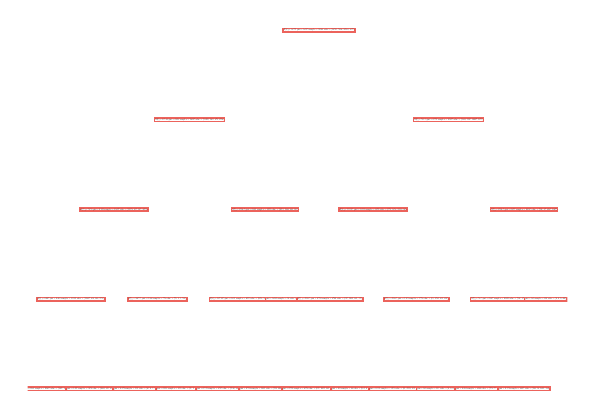
\begin{tikzpicture}

\definecolor{darkgray176}{RGB}{176,176,176}
\definecolor{tomato2369992}{RGB}{236,99,92}

\begin{axis}[
hide x axis,
hide y axis,
tick align=outside,
tick pos=left,
x grid style={darkgray176},
xmin=0, xmax=1,
xtick style={color=black},
y grid style={darkgray176},
ymin=0, ymax=1,
ytick style={color=black}
]
\draw (axis cs:0.04,0.1) node[
  scale=0.0727700654015225,
  fill=white,
  draw=tomato2369992,
  line width=0.6pt,
  inner sep=3.6pt,
  text=black,
  rotate=0.0,
  align=center
]{gini = 0.186
samples = 10265
value = [9205, 21, 10, 1029]};
\draw (axis cs:0.12,0.1) node[
  scale=0.0727700654015225,
  fill=white,
  draw=tomato2369992,
  line width=0.6pt,
  inner sep=3.6pt,
  text=black,
  rotate=0.0,
  align=center
]{gini = 0.495
samples = 3054
value = [2082, 213, 232, 527]};
\draw (axis cs:0.2,0.1) node[
  scale=0.0727700654015225,
  fill=white,
  draw=tomato2369992,
  line width=0.6pt,
  inner sep=3.6pt,
  text=black,
  rotate=0.0,
  align=center
]{gini = 0.471
samples = 139
value = [46, 0, 3, 90]};
\draw (axis cs:0.28,0.1) node[
  scale=0.0727700654015225,
  fill=white,
  draw=tomato2369992,
  line width=0.6pt,
  inner sep=3.6pt,
  text=black,
  rotate=0.0,
  align=center
]{gini = 0.112
samples = 439
value = [25, 1, 0, 413]};
\draw (axis cs:0.36,0.1) node[
  scale=0.0727700654015225,
  fill=white,
  draw=tomato2369992,
  line width=0.6pt,
  inner sep=3.6pt,
  text=black,
  rotate=0.0,
  align=center
]{gini = 0.539
samples = 2595
value = [1548, 824, 59, 164]};
\draw (axis cs:0.44,0.1) node[
  scale=0.0727700654015225,
  fill=white,
  draw=tomato2369992,
  line width=0.6pt,
  inner sep=3.6pt,
  text=black,
  rotate=0.0,
  align=center
]{gini = 0.722
samples = 1461
value = [504, 404, 167, 386]};
\draw (axis cs:0.52,0.1) node[
  scale=0.0727700654015225,
  fill=white,
  draw=tomato2369992,
  line width=0.6pt,
  inner sep=3.6pt,
  text=black,
  rotate=0.0,
  align=center
]{gini = 0.709
samples = 2672
value = [615, 1069, 681, 307]};
\draw (axis cs:0.6,0.1) node[
  scale=0.0727700654015225,
  fill=white,
  draw=tomato2369992,
  line width=0.6pt,
  inner sep=3.6pt,
  text=black,
  rotate=0.0,
  align=center
]{gini = 0.0
samples = 28
value = [0, 0, 0, 28]};
\draw (axis cs:0.68,0.1) node[
  scale=0.0727700654015225,
  fill=white,
  draw=tomato2369992,
  line width=0.6pt,
  inner sep=3.6pt,
  text=black,
  rotate=0.0,
  align=center
]{gini = 0.331
samples = 3459
value = [61, 2789, 431, 178]};
\draw (axis cs:0.76,0.1) node[
  scale=0.0727700654015225,
  fill=white,
  draw=tomato2369992,
  line width=0.6pt,
  inner sep=3.6pt,
  text=black,
  rotate=0.0,
  align=center
]{gini = 0.0
samples = 113
value = [0, 0, 0, 113]};
\draw (axis cs:0.84,0.1) node[
  scale=0.0727700654015225,
  fill=white,
  draw=tomato2369992,
  line width=0.6pt,
  inner sep=3.6pt,
  text=black,
  rotate=0.0,
  align=center
]{gini = 0.214
samples = 8124
value = [378, 55, 7174, 517]};
\draw (axis cs:0.92,0.1) node[
  scale=0.0727700654015225,
  fill=white,
  draw=tomato2369992,
  line width=0.6pt,
  inner sep=3.6pt,
  text=black,
  rotate=0.0,
  align=center
]{gini = 0.354
samples = 2295
value = [128, 32, 1811, 324]};
\draw (axis cs:0.08,0.3) node[
  scale=0.0727700654015225,
  fill=white,
  draw=tomato2369992,
  line width=0.6pt,
  inner sep=3.6pt,
  text=black,
  rotate=0.0,
  align=center
]{X[1] <= 0.005
gini = 0.268
samples = 13319
value = [11287, 234, 242, 1556]};
\draw (axis cs:0.24,0.3) node[
  scale=0.0727700654015225,
  fill=white,
  draw=tomato2369992,
  line width=0.6pt,
  inner sep=3.6pt,
  text=black,
  rotate=0.0,
  align=center
]{X[5] <= 1067.5
gini = 0.228
samples = 578
value = [71, 1, 3, 503]};
\draw (axis cs:0.4,0.3) node[
  scale=0.0727700654015225,
  fill=white,
  draw=tomato2369992,
  line width=0.6pt,
  inner sep=3.6pt,
  text=black,
  rotate=0.0,
  align=center
]{X[2] <= 127.415
gini = 0.631
samples = 4056
value = [2052, 1228, 226, 550]};
\draw (axis cs:0.48,0.3) node[
  scale=0.0727700654015225,
  fill=white,
  draw=tomato2369992,
  line width=0.6pt,
  inner sep=3.6pt,
  text=black,
  rotate=0.0,
  align=center
]{gini = 0.021
samples = 94
value = [1, 0, 0, 93]};
\draw (axis cs:0.56,0.3) node[
  scale=0.0727700654015225,
  fill=white,
  draw=tomato2369992,
  line width=0.6pt,
  inner sep=3.6pt,
  text=black,
  rotate=0.0,
  align=center
]{X[5] <= 2502.5
gini = 0.712
samples = 2700
value = [615, 1069, 681, 335]};
\draw (axis cs:0.72,0.3) node[
  scale=0.0727700654015225,
  fill=white,
  draw=tomato2369992,
  line width=0.6pt,
  inner sep=3.6pt,
  text=black,
  rotate=0.0,
  align=center
]{X[5] <= 2502.5
gini = 0.369
samples = 3572
value = [61, 2789, 431, 291]};
\draw (axis cs:0.88,0.3) node[
  scale=0.0727700654015225,
  fill=white,
  draw=tomato2369992,
  line width=0.6pt,
  inner sep=3.6pt,
  text=black,
  rotate=0.0,
  align=center
]{X[5] <= 52.5
gini = 0.247
samples = 10419
value = [506, 87, 8985, 841]};
\draw (axis cs:0.96,0.3) node[
  scale=0.0727700654015225,
  fill=white,
  draw=tomato2369992,
  line width=0.6pt,
  inner sep=3.6pt,
  text=black,
  rotate=0.0,
  align=center
]{gini = 0.0
samples = 206
value = [0, 0, 0, 206]};
\draw (axis cs:0.16,0.5) node[
  scale=0.0727700654015225,
  fill=white,
  draw=tomato2369992,
  line width=0.6pt,
  inner sep=3.6pt,
  text=black,
  rotate=0.0,
  align=center
]{X[5] <= 525.0
gini = 0.309
samples = 13897
value = [11358, 235, 245, 2059]};
\draw (axis cs:0.44,0.5) node[
  scale=0.0727700654015225,
  fill=white,
  draw=tomato2369992,
  line width=0.6pt,
  inner sep=3.6pt,
  text=black,
  rotate=0.0,
  align=center
]{X[5] <= 2502.5
gini = 0.641
samples = 4150
value = [2053, 1228, 226, 643]};
\draw (axis cs:0.64,0.5) node[
  scale=0.0727700654015225,
  fill=white,
  draw=tomato2369992,
  line width=0.6pt,
  inner sep=3.6pt,
  text=black,
  rotate=0.0,
  align=center
]{X[1] <= 563.315
gini = 0.569
samples = 6272
value = [676, 3858, 1112, 626]};
\draw (axis cs:0.92,0.5) node[
  scale=0.0727700654015225,
  fill=white,
  draw=tomato2369992,
  line width=0.6pt,
  inner sep=3.6pt,
  text=black,
  rotate=0.0,
  align=center
]{X[5] <= 2502.5
gini = 0.273
samples = 10625
value = [506, 87, 8985, 1047]};
\draw (axis cs:0.3,0.7) node[
  scale=0.0727700654015225,
  fill=white,
  draw=tomato2369992,
  line width=0.6pt,
  inner sep=3.6pt,
  text=black,
  rotate=0.0,
  align=center
]{X[1] <= 135.22
gini = 0.418
samples = 18047
value = [13411, 1463, 471, 2702]};
\draw (axis cs:0.78,0.7) node[
  scale=0.0727700654015225,
  fill=white,
  draw=tomato2369992,
  line width=0.6pt,
  inner sep=3.6pt,
  text=black,
  rotate=0.0,
  align=center
]{X[1] <= 783.3
gini = 0.574
samples = 16897
value = [1182, 3945, 10097, 1673]};
\draw (axis cs:0.54,0.9) node[
  scale=0.0727700654015225,
  fill=white,
  draw=tomato2369992,
  line width=0.6pt,
  inner sep=3.6pt,
  text=black,
  rotate=0.0,
  align=center
]{X[1] <= 385.71
gini = 0.695
samples = 34944
value = [14593, 5408, 10568, 4375]};
\end{axis}

\end{tikzpicture}
